\documentclass[tikz,border=3pt]{standalone}

\usepackage{tikz}
\usetikzlibrary{arrows.meta,calc,positioning}

\definecolor{neutral}{HTML}{263640}
\definecolor{lightneutral}{HTML}{6B7A84}
\definecolor{signcolor}{HTML}{7C3AED}
\definecolor{significandcolor}{HTML}{0F766E}
\definecolor{normalizecolor}{HTML}{A16207}
\definecolor{exponentcolor}{HTML}{2563EB}
\definecolor{roundcolor}{HTML}{BE185D}

\tikzset{
  block/.style={
    draw=#1,
    fill=#1!7,
    rounded corners=1.2pt,
    line width=1.15pt,
    minimum height=1.05cm,
    inner xsep=8pt,
    inner ysep=6pt,
    align=center,
    font=\sffamily\normalsize
  },
  wire/.style={
    draw=#1,
    line width=1.15pt,
    line cap=round,
    line join=round,
    -{Latex[length=2.0mm,width=1.3mm]}
  },
  control/.style={
    draw=#1,
    line width=1.05pt,
    dashed,
    line cap=round,
    line join=round,
    -{Latex[length=1.9mm,width=1.25mm]}
  },
  port/.style={font=\ttfamily\large, text=neutral},
  signal/.style={font=\sffamily\small, text=#1, fill=white, inner sep=2pt}
}

\begin{document}
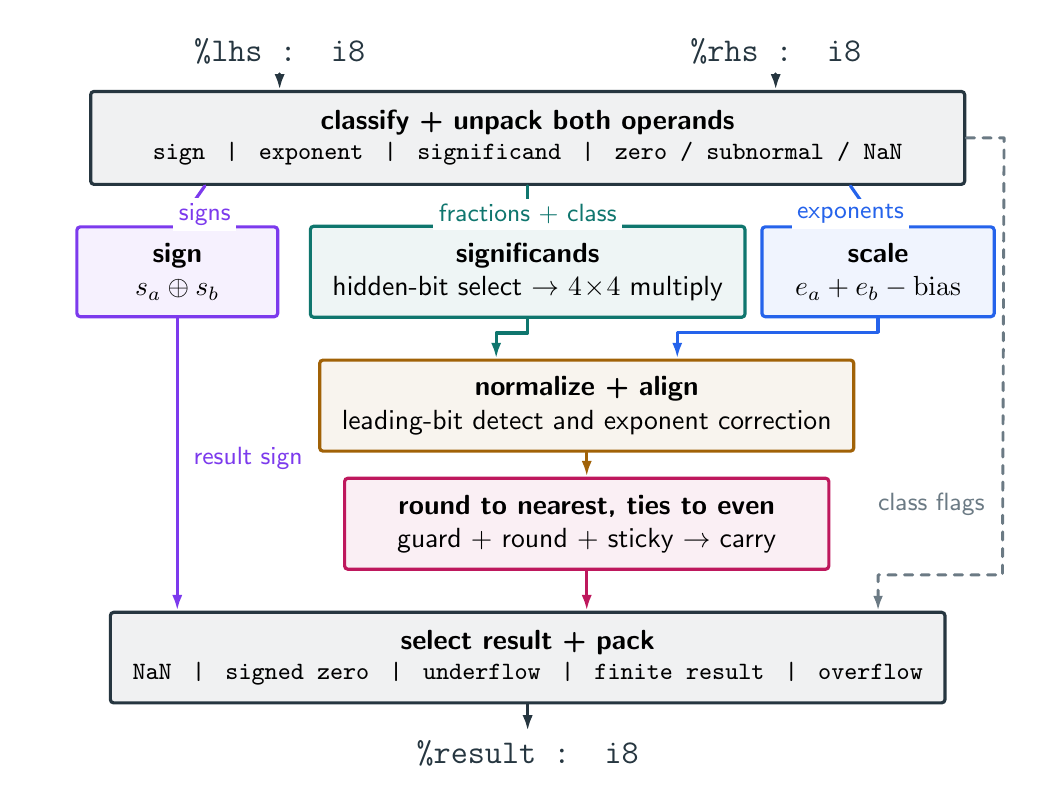
\begin{tikzpicture}
  \path[use as bounding box] (-6.35,-4.75) rectangle (6.35,4.75);

  \node[port] (lhs) at (-3.15,4.45) {\%lhs : i8};
  \node[port] (rhs) at ( 3.15,4.45) {\%rhs : i8};

  \node[block=neutral, minimum width=11.1cm, minimum height=1.18cm]
    (decode) at (0,3.35)
    {\textbf{classify + unpack both operands}\\[-1pt]
     \ttfamily\small sign \;|\; exponent \;|\; significand \;|\; zero / subnormal / NaN};

  \node[block=signcolor, minimum width=2.55cm] (sign) at (-4.45,1.65)
    {\textbf{sign}\\$s_a \oplus s_b$};
  \node[block=significandcolor, minimum width=4.25cm] (multiply) at (0,1.65)
    {\textbf{significands}\\hidden-bit select $\rightarrow$ $4\!\times\!4$ multiply};
  \node[block=exponentcolor, minimum width=2.95cm] (scale) at (4.45,1.65)
    {\textbf{scale}\\$e_a + e_b - \mathrm{bias}$};

  \node[block=normalizecolor, minimum width=6.15cm] (normalize) at (0.75,-0.05)
    {\textbf{normalize + align}\\leading-bit detect and exponent correction};
  \node[block=roundcolor, minimum width=6.15cm] (round) at (0.75,-1.55)
    {\textbf{round to nearest, ties to even}\\guard + round + sticky $\rightarrow$ carry};

  \node[block=neutral, minimum width=10.55cm, minimum height=1.15cm]
    (select) at (0,-3.25)
    {\textbf{select result + pack}\\[-1pt]
     \ttfamily\small NaN \;|\; signed zero \;|\; underflow \;|\; finite result \;|\; overflow};
  \node[port] (result) at (0,-4.47) {\%result : i8};

  \draw[wire=neutral] (lhs.south) -- ($(decode.north)+(-3.15,0)$);
  \draw[wire=neutral] (rhs.south) -- ($(decode.north)+( 3.15,0)$);

  \draw[wire=signcolor] ($(decode.south)+(-4.1,0)$) -- (sign.north);
  \draw[wire=significandcolor] (decode.south) -- (multiply.north);
  \draw[wire=exponentcolor] ($(decode.south)+(4.1,0)$) -- (scale.north);
  \node[signal=signcolor] at (-4.1,2.38) {signs};
  \node[signal=significandcolor] at (0,2.38) {fractions + class};
  \node[signal=exponentcolor] at (4.1,2.38) {exponents};

  \draw[wire=significandcolor] (multiply.south) -- ++(0,-0.18)
    -| ($(normalize.north)+(-1.15,0)$);
  \draw[wire=exponentcolor] (scale.south) -- ++(0,-0.18)
    -| ($(normalize.north)+(1.15,0)$);
  \draw[wire=normalizecolor] (normalize.south) -- (round.north);
  \draw[wire=roundcolor] (round.south) -- ($(select.north)+(0.75,0)$);

  \draw[wire=signcolor] (sign.south) -- ($(select.north)+(-4.45,0)$);
  \node[signal=signcolor, anchor=west] at (-4.32,-0.72) {result sign};

  \draw[control=lightneutral] (decode.east) -- ++(0.48,0)
    -- (6.03,-2.20) -- (4.45,-2.20)
    -- ($(select.north)+(4.45,0)$);
  \node[signal=lightneutral, anchor=east] at (5.88,-1.30) {class flags};

  \draw[wire=neutral] (select.south) -- (result.north);
\end{tikzpicture}
\end{document}
